\chapter{Implementation}
\label{sec:implementation}

% Hier greift man einige wenige, interessante Gesichtspunkte der
% Implementierung heraus. Das Kapitel darf nicht mit Dokumentation oder
% gar Programmkommentaren verwechselt werden. Es kann vorkommen, daß
% sehr viele Gesichtspunkte aufgegriffen werden müssen, ist aber nicht
% sehr häufig. Zweck dieses Kapitels ist einerseits, glaubhaft zu
% machen, daß man es bei der Arbeit nicht mit einem "Papiertiger"
% sondern einem real existierenden System zu tun hat. Es ist sicherlich
% auch ein sehr wichtiger Text für jemanden, der die Arbeit später
% fortsetzt. Der dritte Gesichtspunkt dabei ist, einem Leser einen etwas
% tieferen Einblick in die Technik zu geben, mit der man sich hier
% beschäftigt. Schöne Bespiele sind "War Stories", also Dinge mit denen
% man besonders zu kämpfen hatte, oder eine konkrete, beispielhafte
% Verfeinerung einer der in Kapitel 3 vorgestellten Ideen. Auch hier
% gilt, mehr als 20 Seiten liest keiner, aber das ist hierbei nicht so
% schlimm, weil man die Lektüre ja einfach abbrechen kann, ohne den
% Faden zu verlieren. Vollständige Quellprogramme haben in einer Arbeit
% nichts zu suchen, auch nicht im Anhang, sondern gehören auf Rechner,
% auf denen man sie sich ansehen kann.

In this chapter implementation details will be discussed.
It elaborates on the hurdles that were encountered during the development of the load balancer and how they were overcome.
Most of the problems discussed root in the design of a microkernel-based operating system, which is comparable to a distributed system, and the scheduler, which is often designed to be part of the kernel, is now implemented in user space.

\section{Scheduling Proxy}
\label{sec:impl:proxy}

The scheduling proxy handles all functionality that is exposed by the scheduler interface but mainly \texttt{run\_thread()}.
Because the function itself is straightforward, only the most interesting details are investigated further in the following section.
The proxy is the entity in the load balancer that maintains the addition of new threads into the bookkeeping structures and, therefore, their capabilities.
They are one of the main security features L4Re is built upon and require special handling.

\subsection{Capability Slots}
\label{sec:impl:cap-slots}

Capabilities are the primitive to control access rights to objects in L4Re.
To prevent applications from maliciously manipulating their own domain of access, capabilities are managed by the application but maintained in kernel space by the kernel.
The app only has access to a so-called capability table that allows the invocation of entries to request the kernel to execute an operation with the object behind the specified capability.
Thus, the userland only operates on capability table slots, as can be seen in Figure~\ref{fig:cap-table}.

\begin{figure}[h]
	\centering
	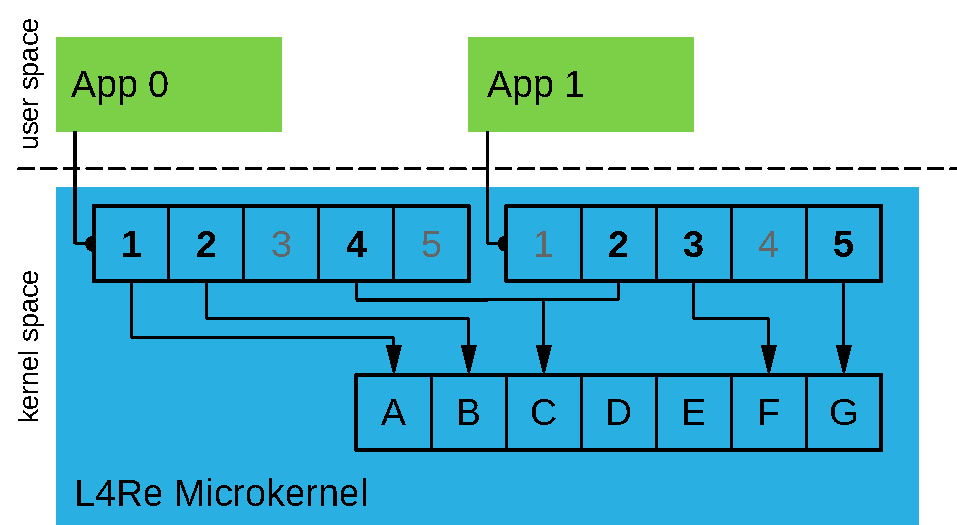
\includegraphics[width=0.7\linewidth]{images/capability_table.pdf}
	\caption{L4Re capability tables and entries (indices) of applications referencing kernel objects (characters) in kernel space.}
	\label{fig:cap-table}
\end{figure}

The moment the scheduling proxy receives a new thread capability via \texttt{run\_thread()}, it needs to check if it already tracks that thread.
The proxy does not have access to the actual capability objects but can only request the kernel to act upon a given index of the capability table.
This table has a receive slot (index) that determines where the next incoming capability is written to.
The moment the scheduling proxy decides to add a thread into its bookkeeping, it takes ownership of the thread's capability.
When doing so, the receive slot must be moved to a new unoccupied table index; otherwise, the next call of \texttt{run\_thread()} will overwrite the previously stored capability.
An overwritten capability would thus lead to threads the proxy took ownership of but cannot access anymore, making it unable to migrate them in the future.
To solve this leakage of dangling threads, the proxy needs to call \texttt{realloc\_rcv\_cap()} after taking ownership of an incoming capability.
This moves the table entry to an empty slot where new capabilities can be received.
Because memory is finite, the capability table is limited in size, and \texttt{realloc\_rcv\_cap()} will return an error when it runs out of empty capability slots.
This error indicates that the table is fully occupied and the load balancer is not capable of handling any more new threads because no empty slot is left in the table.
This scenario does not present a practical limitation, as the table size can be increased up to thousands or millions of entries.

\subsection{Access Rights}

The scheduling proxy only acts upon indices in the table instead of capabilities themselves, which means that it is not able to determine if the capabilities stored in two slots point to the same object.
The L4Re microkernel provides a system call to determine if two capabilities are equal called \texttt{cap\_equal()}.
It compares the capabilities stored in the specified table entries and returns a boolean value.
This mechanism allows the scheduling proxy to check if the received capability by \texttt{run\_thread()} is unique or already tracked.
The first problem exposed by this approach is that identifying a thread requires $n$ system calls when $n$ threads are already tracked, just to compare capabilities.
This solution could be improved by batching the requests to the kernel; however, Section~\ref{sec:overhead-analysis} will show that the overhead of the scheduling proxy can be ignored and does not pose a scalability problem.
The second, much more serious problem that results in erroneous behavior if not handled correctly is that capabilities are the union of an object pointer and the assigned rights to that object.
Two capabilities referencing the same thread but with different access rights are not considered equal.
This poses a problem for the load balancer because applications can call \texttt{run\_thread} on the same thread multiple times.
The \texttt{pthread} library used to create threads invokes \texttt{run\_thread} with a reduced set of access rights.
Although the design of \texttt{cap\_equal()} is absolutely correct, this behavior will break the bookkeeping structures of the load balancer.

To avoid this all at once, the kernel was extended by the \texttt{cap\_equal\_no\_rights()} system call.
It still compares two capabilities for equality but does not regard the associated access rights as only object references.
This way, the scheduling proxy can rely on the assumption that a capability to a thread is unique whenever it points to the same thread.

\section{Monitoring}
\label{sec:monitoring}

\subsection{Dead Threads}

In Section~\ref{sec:des:proxy}, it was discussed that the scheduling proxy represents the entry point of a tracked thread into the load balancer because it is registered there.
The problem with implementing a scheduling proxy in userland is that it is not not notified when a tracked thread exits the system.
Instead of registering the proxy to be notified by the kernel with an interrupt whenever there is a dead thread in its domain, it is easier and more efficient to extend a mechanism already in use.
The \texttt{stats\_time()} system call needs to be invoked for every tracked thread each monitoring interval (see Section~\ref{sec:des:monitoring}).
An invocation with the capability of a thread that has already left the system results in an IPC error message.
This signals to the monitoring thread that it can now delete the affected thread from the bookkeeping structures of the load balancer.

The deletion of a dead thread needs to be managed properly to avoid corrupting the bookkeeping because there are multiple tracking data structures referencing threads.
Tracked threads reside in their appropriate run queue and thread group, defining the allowed CPU scheduling set (see Section~\ref{sec:thread-groups}).
Because the monitoring infrastructure uses run queues to iterate through threads for probing, they have been made the governing data structure.
A dead thread is deleted from its run queue, and the destructor removes the thread through back references from its assigned scheduling group.
If a thread group runs empty the moment a thread deregisters from it, the group triggers its own removal from the set of groups.

\subsection{Thread Probing}
\label{sec:probing}

Monitoring threads iterate all threads contained in the shadow run queue assigned to the CPU they are running on (see Section~\ref{sec:des:monitoring}).
Migrations are not instant, and thus there will be a point in time where a thread is still in migration transition, but the load balancer has already moved the tracked instance to its destination run queue in its bookkeeping.
This leads to complications when the migration is not finished until the next monitoring cycle, as a monitor will try to probe a thread that is not on its CPU yet.
When issuing the system call, the kernel will either look up the information needed right away when the requested thread is on the same CPU as the caller, or it will start a DRQ (see Section~\ref{sec:cross-comm}) on behalf of the caller to the requested thread.
This behavior poses a problem to the monitor because if a thread is still in migration transition, the probing request will not be executed with the priority of the monitor anymore but with the priority of the requested thread.
In most cases, this will lead to a scenario that is known as \enquote{priority inversion.}
The monitor with a high priority blocks on a low priority thread, which is then preempted by a medium priority thread on the destination CPU.
Inevitably inverting the priority of the monitor because it is delayed by the medium-priority thread for an arbitrary amount of time despite having higher priority~\cite{priority-inheritance-protocols}.
Further, system calls cannot be requested using timeouts; therefore, the monitor would be stuck until the requested thread handled the DRQ.
To avoid this interaction, the \texttt{stats\_time()} system call was modified to return an error code instead of executing a DRQ.
It comes at the cost of working with outdated information for that tracked thread and monitoring cycle but assures that the load balancer infrastructure cannot block during system calls.

\subsection{Timing}

Numerous components of the load balancer require precise and synchronized timing to function correctly.
The commander and monitors use absolute timeouts to orchestrate themselves (see Section~\ref{sec:abs-timeouts}).
The proxy and commander use precise timing to identify monitors whose information is outdated, and the monitoring threads themselves rely on it because of the CPU idle time and thread probing.
To provide exact timing to the load balancer, the L4Re microkernel needs to support \texttt{FINE\_GRAINED\_CPUTIME}.
When enabled, the kernel then calculates the exact CPU usage of a thread on every context switch instead of \si{\ms} granularity.
Additionally, the \texttt{SYNC\_CLOCK} option should to be set, which requires \texttt{HAS\_SYNC\_CLOCK} to ensure that all CPUs can read the same system time.
It has to be mentioned that \texttt{SYNC\_CLOCK} could lead to complications when operating on processors that have more than one hardware socket.
Without both features activated, the time received by the \texttt{idle\_time()} system call and the value returned by \texttt{l4\_kip\_clock(l4\_kip())} deviated heavily, leading to incorrect results when calculating the CPU load from idle and passed time.

\iffalse
% This is a debatable topic and should not be used
\section{Priority Usage}

Section~\ref{sec:insight-prio} discusses the idea that the load balancer threads should assign themselves the highest priority possible.
In the default priority band, this would translate to 255, which is a reserved priority for important tasks only.
The only instances with that priority are the root task Moe, the pager, and the interrupt handler of each application ITAS and software interrupt requests (SW IRQs).
The one monitor per CPU, the scheduling proxy on CPU1, and the commander on either CPU1 or CPU2 would then compete against Moe and ITAS in round-robin scheduling or during message delivery of IPC communication with SW IRQs at the same receiver.
Interrupt delivery and its handling are assumed to be as fast as possible to reduce interrupt latency.
In a priority-based operating system, this principle is followed through as well, but the thread with the highest priority gets to monopolize the CPU anyway.
Hence, even if the software IRQ is delivered and handled with the highest importance, an application with a lower priority than the load balancer will be suspended when monitoring or rebalancing is taking place.
Therefore, it does not matter to the application if the load balancer is competing with those or not because it will be preempted nevertheless.
Further, SW IRQs would only compete with IPC messages of the load balancer if they had the same destination, but all load balancer components have self-contained communication, meaning they only exchange IPC with themselves or make system calls.
Hence, they would not interfere with SW IRQs in the first place, leading to the decision that a priority of 255 is safe to use for the load balancing components.

Although not a disturbance within the scope of this work, it should be investigated and discussed for future systems if the load balancer's importance requires it to use priority 255 or if 254 would be sufficient as well.
This would make it inferior to Moe on CPU0 but would adhere to the guideline of having the maximum priority reserved.

\fi

\section{Load Balancing}
\label{sec:impl:loba}

\subsection{Tracking Preemptions}

In Section~\ref{sec:des:loba}, the metric \texttt{vload} was introduced, allowing for robust CPU monitoring.
The preemptions, the thread's demand, and ultimately the virtual load metric are tracked using a sliding window approach.
For this an array structure is needed that captures the previous $n$ preemptions or yields of the thread.	
The information is provided by the kernel, and therefore it needs to track such an array for every thread in the system.
It is preferred to solve this problem with a stateless and memory-efficient approach.
An actual array paired with a pointer to create a looping ring buffer would be a viable implementation for the job but is way too complex for the actual task.
Ultimately, the sliding window needs to store zeros and ones, which can be done much more space- and time-efficiently by a single machine word.
When the timer tick hits or the thread yields, the kernel can simply shift the machine word left once and add the new decision at the least significant bit.
In doing so, this gets rid of an actual array, which would also be more difficult to transfer via the system call than a single register is.

\subsection{Calculating Demand}

Every bit of the preemption machine word adds to a demand value.
The older a bit is in time, the lower its added value is.
This concept assumes that information further in the past has less correlation with what will happen in the future.
For determining the half-life of the preemption bits, the Linux scheduler was considered.
It uses aging when calculating its virtual runtime, and information that is \SI{32}{\ms} in the past only accounts for half its original weight.

Hence, the demand is calculated using the sum of a geometric sequence.
\[
S_n = x_1 y^1 + x_2 y^2 + x_3 y^3 + \dots + x_n y^n = \sum_{k=1}^{n} x_k y^k
\]
Using a machine word also comes in handy when calculating this sum.
Instead of iterating an array, the machine word can be used as the condition of a while loop, shifting the register each iteration; therefore, the loop ends when the machine word is all zeros, sparing unnecessary iterations.
Further, the half-life of \SI{32}{\ms} makes the final bits of no influence, as their contribution is marginal.
This allows for masking the preemption machine word beforehand to only be left with significant bits and exiting the while loop early after necessary parts were computed.

\subsection{Rebalancing}
\label{sec:rebalancing}

Load balancing is kept simple by calculating the average vload over all CPUs and then determining an upper and lower bound by adding or subtracting 20\,\% from the average.
Thereby, the \texttt{vload} of a CPU is the sum of the \texttt{vload} of its run queue threads divided by the performance factor of this CPU.
All CPUs above the calculated upper bound and at 90\% actual CPU load are considered overloaded, and all below the lower bound are underloaded.
If an overloaded CPU only has one thread in its run queue, it is skipped, except for CPU0, as the L4Re infrastructure threads like Moe are placed there.
Per overloaded source CPU, one thread will be moved to an underloaded destination CPU.
This decision is made using a scoring function that considers the destination's load, the thread's \texttt{vload} and migration cost, and the destination's capacity for the thread's priority (1 minus the CPU usage of threads of higher or equal priority).
The cost of a migration is estimated by using the CPU time a thread consumed during the previous monitoring interval, as it is assumed that a high CPU usage correlates with caches still being warm. 
This metric is taken into account because it is expensive to reload cache content at the destination CPU.
A migration of a thread that would overload the destination is disregarded.
Also the \texttt{vload} of every planned migration is projected onto the \texttt{vload} of the destination CPU to prevent pile up on a CPU that seems favorable.
The migrations with the best scores are stored and executed after the rebalancing algorithm is done.

\paragraph{Key Insight.}
\label{sec:insight-placement}

There will be a hidden load the load balancer cannot measure because it is caused by threads that are not tracked by its bookkeeping, including the load balancer itself.
The most common example for this phenomenon is Moe because it is needed to launch a load balancer instance and can therefore not use it as its scheduler.
It is always located on CPU0 and activates occasionally when system-level background tasks need to be done, like allocating or freeing memory; thus, it does not constantly cause load but rather does so in bursts. 
This behavior is the reason why the scheduler proxy is moved to CPU1 and the commander to CPU2 (if available) so they do not get interrupted by those occasional spikes in hidden CPU time consumption.

\section{Thread Groups}

It is crucial to provide mutually exclusive CPU sets to vCPUs when their thread groups receive a reassignment of allowed physical CPUs (see Section~\ref{sec:thread-groups}).
This separation is the reason why every group needs to track all other groups it is disjunctive with.
When constructing a new CPU assignment, all those tracked groups need to be regarded to assure that vCPUs do not end up on the same physical CPU.
The problem is a simpler version of the bin packing problem and can therefore be efficiently shortcut~\cite{binpacking}.
The approach of this work uses the \texttt{std::bitset<N>} struct from the standard library, with N being the maximal number of CPUs the load balancer is able to detect.
It is used to represent the CPU set as a bitmap, where each bit corresponds to exactly one physical CPU.
The bitset is a data structure whose size is known at compile time, making it fast, as boolean operators are supported.

Calculating the new CPU assignment requires a bitset with all physically available CPUs.
It is stripped of all bits that are set in disjunctive groups' bitsets, leaving all available CPUs from which the group can now choose.
The calculation can be done efficiently by applying a bitwise \texttt{AND} on the available and inverse disjunctive bitsets iteratively.
The affected group can then select CPUs from this available set until its own CPU demand is satisfied, or in other words, until the population count of the assigned set is equal to the population count of the original CPU set.
The selection process can implement any policy.
For this work the CPUs with the lowest \texttt{vload} are chosen first.
The calculation and assignment process is then carried through for all groups in ascending order of the population count of the originally assigned CPU sets.

\section{Thread Safety}

The load balancer is designed as a multithreaded application working on shared data structures.
When resources are operated using multiple threads, their write accesses need to be mutually exclusive to avoid corrupting the state of the data structure.
The most common primitive operating system provides for locking with a mutex (lock).
The thread that currently holds the mutex can therefore safely read and modify structures like the thread groups and run queues while other threads trying to acquire the lock are blocked.
For reading and writing simple state structures such as tracked threads or CPU states, this would introduce unnecessary overhead without yielding any benefits compared to using atomic operations provided by all architectures.
Only when the size of the attribute that needs to be protected disallows the use of atomics, a mutex is again used to make that attribute thread safe.
The two mechanisms of atomic operations and mutex locking allow for concurrent access of the shared structures.

\section{Distributed System in Userland}
\label{sec:distributed-system}

Section~\ref{sec:commander} states that the design of the load balancing component on top of the L4Re microkernel-based architecture leads to a distributed system.
The scheduling proxy, commander, and all monitors can be preempted at any time.
Therefore, they require an implementation that does not halt the entire load balancer just because one thread of the monitoring infrastructure was preempted.
The load balancer is designed to orchestrate threads on multiple CPUs; hence, it also needs to scale well with a rising number of physical cores.
This challenge can be taken on with an asynchronous approach.

The only threads issuing migrations and, therefore, making decisions are the scheduling proxy and commander.
If either one should be preempted, that is simply user-space load balancing, which is undesirable but unavoidable.
What should be avoided is that a monitoring thread blocks either the proxy or the commander, making them unable to make an informed placement decision.
This scenario can happen because of the introduction of thread-safe accesses and locks.
When a monitor is suspended while iterating its CPU's run queue, it still holds the run queue's mutex.
If the commander or proxy then tries to insert a thread into that run queue, they will block because they need to acquire the mutex first.
If all load balancer components are run with the highest system priority, the blocking is bounded, as on the same priority round-robin scheduling is employed, but if this happens with a lower priority, the suspension could be arbitrary.

It is not possible to eliminate this problem entirely without the use of lock- or wait-free implementations.
They usually have a good worst-case but slow average-case performance.
The approach in this thesis (see Section~\ref{sec:abs-timeouts}) makes use of mutex primitives and is therefore prone to special cases of blocking that could lead to scenarios described previously.
The monitors are iterating their assigned run queue to probe all threads on their CPU.
This could lead to the commander being blocked.
The monitor also writes information about the CPU state that includes a timestamp of the update.
Writing the timestamp is the final operation a monitoring thread does in its monitoring cycle before blocking itself with an absolute timeout.
Therefore, the commander can first check the timestamps of all CPU states and verify if their information is outdated.
Once such a state is detected, it is marked by the commander setting its \texttt{vload} to the maximum possible value the attribute can hold.
The commander will proceed rebalancing with all those CPUs that are considered in time.
The same checking mechanism is employed by the scheduling proxy.
However, the scheduling proxy is required to proceed with all CPUs because of thread pinning.
When threads request to be pinned to a specific CPU, the proxy needs to be able to migrate them to that CPU even if it is currently not favorable.

\subsection{Consistent \texttt{vload} Views Through Write Ordering}
\label{sec:vload-updates}

During the development, a centralized and parallel approach has been implemented to update the \text{vload} of the CPU states.
The whole load balancer is implemented and benchmarked with the centralized solution.
The parallel solution was only measured regarding overhead.
During the writing of the thesis, it was determined that the parallel approach does not raise any complications with regard to the multithreaded access pattern.

\paragraph{Centralized.}

In the centralized implementation, the commander iterates all synchronized CPUs to update their \texttt{vload}.
Doing so, it iterates the run queue of every CPU, which would be potentially blocking if unsynchronized CPUs were iterated as well.
As they have been marked beforehand, this does not pose a threat of blocking directly.
There are scenarios that could lead to the commander being blocked by a monitor, but they would need to be constructed carefully and are therefore not regarded as the average case.

The chain of thought for this approach was that proxy and commander need to detect and mark outdated information of CPUs to reduce the chance of blocking.
A marked CPU gets its \texttt{vload} value set to \texttt{UINT64\_MAX} to make it unfavorable for any further selection process.
If the calculation of the CPU's virtual load were carried out by the monitors, they could overwrite this value at arbitrary points in time, also during the rebalancing and the time the proxy picks a CPU on which a thread should run.

The overwrite does not raise any problem with the rebalancing, as the commander only proceeds with synchronized CPUs.
Already marked CPUs could therefore be overwritten without any effect, as their \texttt{vload} is not read until the next monitoring loop.
The scheduling proxy, on the other hand, is not allowed to make any CPU restrictions.
If a thread needs to be pinned, the proxy has to be able to choose from all CPUs, even those that are currently blocked because pinning is a hard constraint.

\paragraph{Parallel.}

The \texttt{vload} can also be updated by the monitors during their probing cycle.
This has the potential to yield a speedup equivalent to the number of CPUs in the system because it eliminates the single commander instance as a bottleneck.
Theoretically, a parallel approach scales better than the centralized counterpart.
The previously stated concern of arbitrary overwrites while the scheduling proxy has to pick a CPU is also unfounded.
All accesses to the \texttt{vload} value of a CPU state are done via atomic reads and writes.
The proxy is not allowed to restrict the CPUs from which it chooses.
However, an overwrite during the selection process is uncomplicated, as it is done via a linear scan.
This leads to only two possible cases where a previously blocked monitor can overwrite a \texttt{vload} entry.
Either the proxy compares the virtual load of the affected CPU or it is overwritten afterward, which would mean that \texttt{UINT64\_MAX} was read as intended.
Otherwise, the \texttt{vload} field is overwritten before the proxy compares it.
Hence, the proxy reads the updated value as if it would not have been marked outdated.
The value cannot change during the comparison, as all accesses are atomic.
Further, the value is read once and potentially written once; therefore, no inconsistent state can be observed by the scheduling proxy.
This approach cannot cause any inconsistencies during the commander loop, as already argued in the previous paragraph, making it the superior solution because of its scalability.

\section{L4Re Particularities}
\label{sec:l4re-particularities}

The following section describes implementation details of the L4Re framework that lead to complications when implementing or validating the load balancer.

\subsection{Migrations}

A migration is always issued at the kernel scheduler, as it is the final instance of any layered scheduling proxy topology.
Although at the kernel level, the scheduler only assigns a new CPU to the affected thread.
The migration is carried out by the thread itself with its own priority.
This mechanism is the reason why thread probing needs to be robust to avoid priority inversion (see Section~\ref{sec:probing}) because the times between migration start and end can be excessive when a thread has low priority.
But migrations in L4Re have a second caveat to them: the thread that issues the migration, which is the scheduling proxy or commander in this work's case, can still block on the \texttt{run\_thread()} system call.
Although part of the kernel, the native scheduler acts on behalf of the thread calling it.
It not only uses the time slice of the caller but also its priority.
Hence, when the commander tries to migrate a thread during the rebalancing process and the destination CPU is currently occupied by a thread with higher priority than the commander, the migration request will block.
The system call will only return when the scheduler can finish its scheduling decision on the destination CPU.

Although unfortunate for the design and execution of the load balancer, both cases are a direct result of the real-time properties of L4Re.
Just because kernel code is called it does not mean that it should be executed with the maximum priority.
Otherwise, malicious low-priority threads could make system calls in high frequency to preempt threads of higher priority, causing continuous cases of priority inversion and violating the priority scheduling design.

\subsection{The CPU0 Problem}
\label{sec:cpu0-problem}

In Section~\ref{sec:rebalancing} it was stated that CPU0 is unfavorable because Moe is placed there and causes hidden load the load balancer cannot measure.
This itself is unpleasant but a fact that needs to be accepted during scheduling in user space.
But the root task Moe has more caveats to itself.
Moe is the only instance in the operating system framework that has access to the kernel output driver handling application console outputs like \texttt{stdout} and \texttt{stderr}.
Serial output is commonly slow; especially the so-called UART (Universal Asynchronous Receiver/Transmitter) driver that Moe uses can take up hundreds of microseconds per character.
The capability of the UART driver can also be handed to other services by Moe, but it will not accelerate the output.
Because of the speed of printing, Moe will monopolize CPU0 with the highest priority whenever any thread makes serial output requests from any CPU.
This behavior inevitably causes priority inversion on CPU0 on a systemwide scale.
That is why printing is considered a debugging feature in L4Re and is therefore omitted on the kernel side for production releases.

Additionally, the same delays can be experienced when memory regions are freed.
Moe is the instance to free memory by unmapping pages when they are no longer needed.
When the affected memory regions are in the range of kibibytes, this will not have a great effect, as pages are commonly in the dimension of 4 KiB.
When the regions that need to be unmapped reach mebibytes, this becomes more complicated because per mebibyte, 256 pages need to be freed.
For applications reaching into GiB territory, this scales poorly, with an unmap call taking up to a few milliseconds.
Although there are super pages that cover 2 MiB instead of 4 KiB, they need to be issued by \texttt{mmap}, which acquires the memory in the first place.
\texttt{Mmap} is the implementation side of the well-known C standard library function \texttt{malloc()}.

This blocking behavior on CPU0 made development more difficult, as \texttt{printf()} statements from any CPU or the exit of memory-heavy applications would disrupt the work of the load balancer.
This behavior led to the placement decision of the scheduling proxy and commander discussed in Section~\ref{sec:insight-placement}.

\section{Optimizations}
\label{sec:impl:optimizations}

The time that the load balancer needs for its monitoring and decision-making is CPU time the balanced application cannot use for its computation.
Therefore, it is desirable to reduce overhead as much as possible in the hot paths of the scheduling proxy, monitors, and commander.
Not only is it important to make efficient design choices for processing data in parallel as described in Section~\ref{sec:abs-timeouts}.
The implementation also needs to be aware of the underlying hardware and its runtime environment.
Both views are required to achieve fast execution times.

\paragraph{Avoid the Floating Point Unit.}

Not only are floating-point calculations more compute-intensive than integer operations, but they also rely on the floating-point unit (FPU) of the CPU.
The FPU is an accelerator that assists the CPU in computing floating-point instructions faster.
Because those operations became more common in modern programs, the unit grew over the years, making it more sophisticated but increasingly costly to maintain.
Every thread needs to maintain its own FPU state, but because of the size of this state, it is expensive to store and load it with every context switch.
Hence, it is desirable to avoid floating-point operations entirely, thereby avoiding the FPU and the need to store and load it on context switches.
This requires the load balancer code to make all calculations with integer values.
In order not to lose precision during division operations, all values are scaled by \texttt{1'000'000}.
This reduces overhead when other threads in the system require the FPU, because the load balancer does not need to compete for FPU ownership with them.

\paragraph{Batched Thread Probing.}
\label{sec:impl:bached-stats}

The extended \texttt{stats\_time()} system call needs to be made for all threads inside a run queue on every CPU.
Resulting in as many kernel entries and exits as there are tracked threads each monitoring cycle.
Compared to a function call, the switch into the kernel is significantly more expensive; hence, it is desired to reduce the number of switches as much as possible.
A batched system call retrieving information about multiple threads at once would do exactly this.
The medium that is used for information exchange during a system call and IPC is the UTCB.
It provides 63 message registers of 64 bits each to transfer data.
The stats for one thread are its CPU time (64-bit), thread state (8-bit), and tracked preemptions (64-bit), resulting in three UTCB message registers used per requested thread.
The UTCB could therefore transfer up to 21 thread stats at once.
\[
\left\lfloor \frac{63 \cdot 64\text{\lbrack bits\rbrack}}{\lceil 64 + 8 + 64\rceil_{64} \text{ \lbrack bits\rbrack}}\right\rfloor = 21
\]
Further, if the tracked preemptions were reduced to 32 bits instead of 64, the required space would reduce to two message registers per thread, increasing the transferred threads to 31.
\[
\left\lfloor \frac{63 \cdot 64\text{\lbrack bits\rbrack}}{\lceil 64 + 8 + 32\rceil_{64} \text{ \lbrack bits\rbrack}}\right\rfloor = 31
\]
Unfortunately, this approach is difficult to implement in the L4Re environment.
The scheduler would be a good choice for executing such a system call, but its remote procedure call framework does not allow for a variable number of received capabilities.
An interface would then need to specify 21 or 31 capabilities for every call, and unused slots would need to be filled with dummy capabilities that then would be treated as an array limiter.
Such a solution seems to overcome the limitations of the framework by making use of bad coding style.
Another approach would be to add this call to the \texttt{Context} or \texttt{Thread} class interface because they do not use the remote procedure call but an IPC framework that allows for variable-capability arrays.
But as thread probing did not represent a bottleneck to the monitoring process, the investigations ended at that point.

\paragraph{Avoid Heap Allocations.}

During each rebalancing run, the commander operates on freshly allocated dynamic data structures.
In doing so, it makes frequent use of memory allocation on the heap, which naturally takes more time than structures that can be allocated on the stack.
Additionally, this could cause page faults that need to be handled, increasing the time spent in the hot path unnecessarily.
To avoid calls to \texttt{malloc}, structures should be allocated on the stack.
It requires the size of all structures to be known at compile time, which usually overestimates the needed space, as governing parameters like the numbers of CPUs can only be determined at runtime, causing internal memory slack space.
Additionally, the use of such structures made the code of the rebalancing method more complicated and did not yield measurable improvements for the scope of this thesis.
Depending on the implementation behind \texttt{malloc}, pages can be reused when they were initially backed by physical memory, making future calls significantly cheaper.
It should also be mentioned that stack memory can also cause page faults.
Therefore, dynamic data structures ended up in the final version of the implementation.

\section{Summary}

This chapter presented the challenges that were faced during the implementation process of the design from Chapter~\ref{sec:design}.
Figure~\ref{fig:impl:overview} visualizes the changes made to the natively provided interfaces of L4Re and the planned design in Figure~\ref{fig:des:overview}.

\begin{figure}
	\centering
	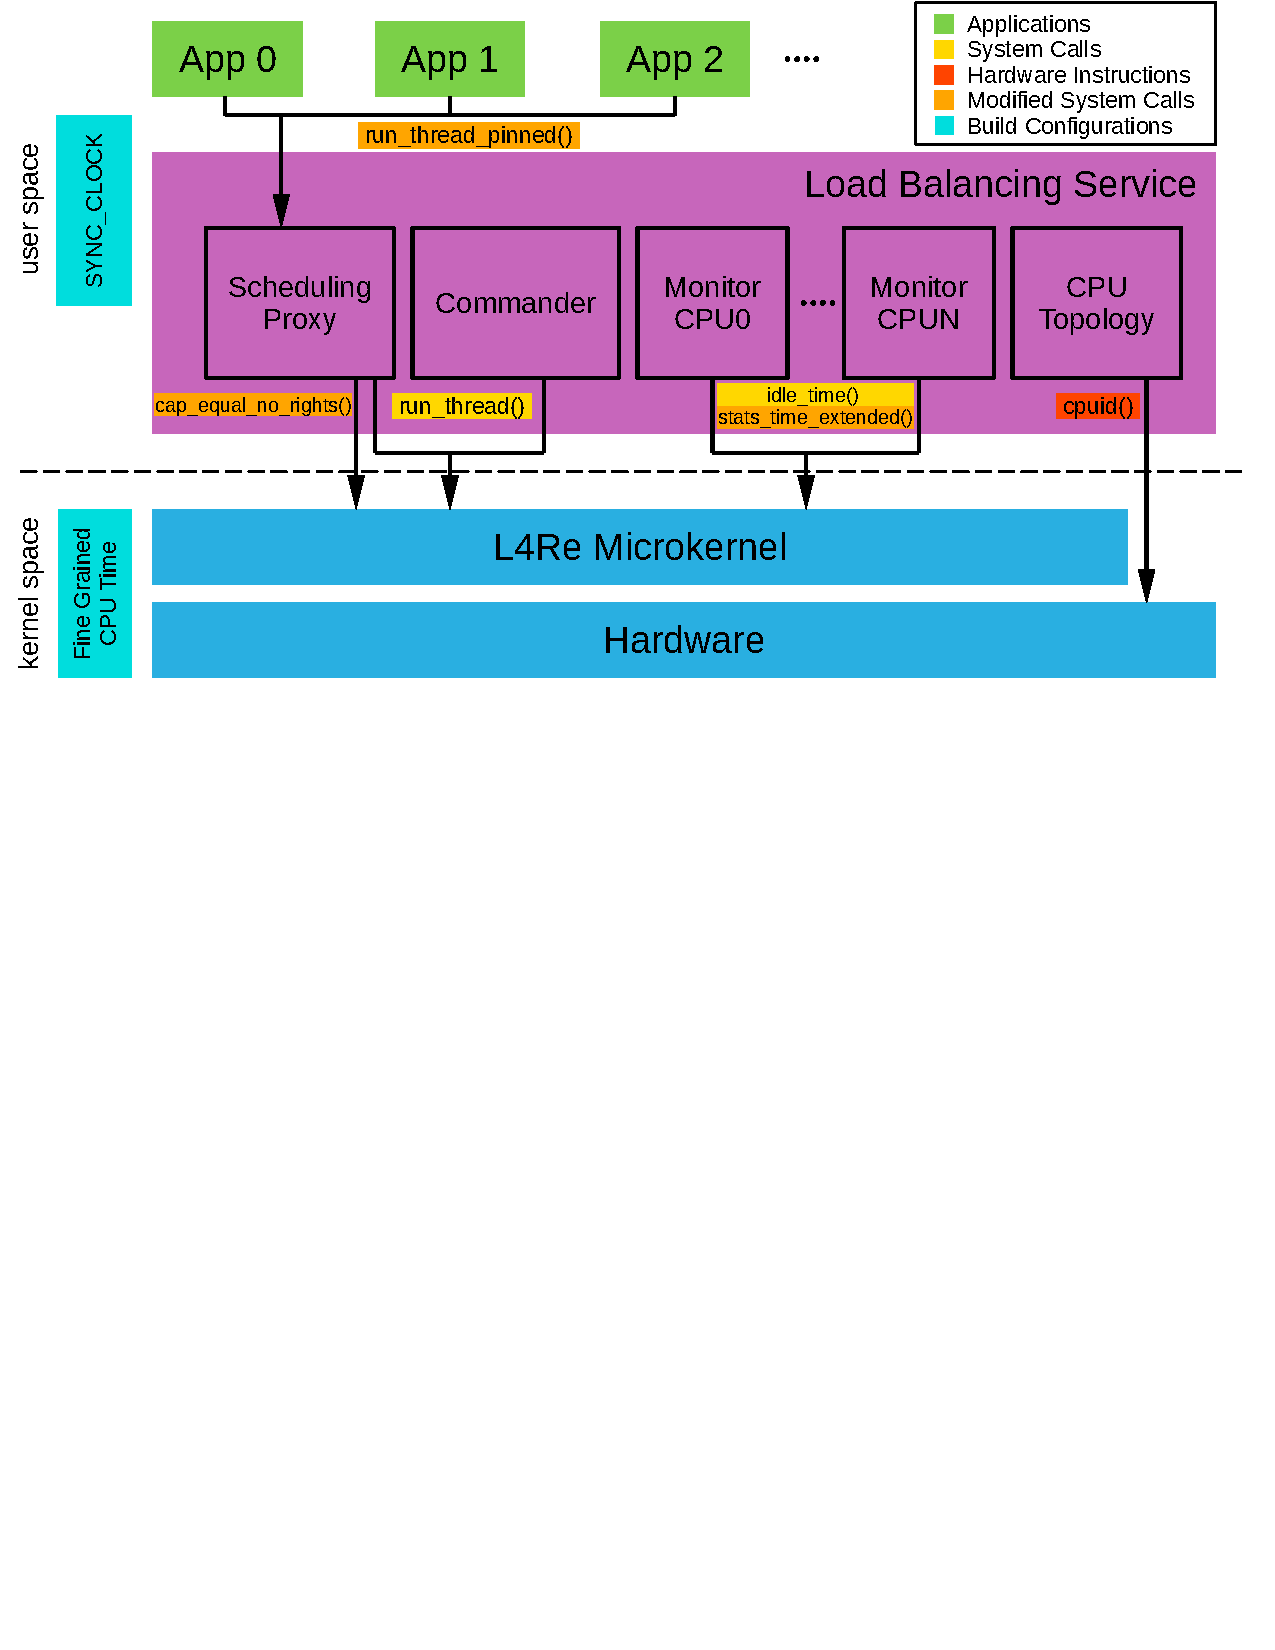
\includegraphics[trim={0 16.5cm 0.3cm 0}, clip, width=\textwidth]{images/arch_overview_impl.pdf}
	\caption{Architecture diagram after the implementation phase. Highlighting modified system calls and required build configurations (compare to Figure~\ref{fig:des:overview}).}
	\label{fig:impl:overview}
\end{figure}

The scheduling proxy (see Section~\ref{sec:proxy}) solved the thread registration process via the extension of the \texttt{cap\_equal()} system call to \texttt{cap\_equal\_no\_rights()}.
During the implementation of the monitoring infrastructure in Section~\ref{sec:monitoring}, the deregistration of dead threads and the probing of live ones were solved by extending \texttt{stats\_time()} to \texttt{stats\_time\_extended()}.
This extension makes the monitor able to read the CPU usage, thread state, and preemption history of a thread.
Additionally, the essential user land and kernel build configurations of \texttt{SYNC\_CLOCK} and \texttt{Fine Grained CPU Time} were added in turquoise in Figure~\ref{fig:impl:overview} as 'Build Configurations'.
In Section~\ref{sec:impl:loba}, thread placement is built on top of the \texttt{vload} metric that is derived from the preemption history of a thread.
Shared data structures like the thread groups that are used for placement constraints required thread-safe access patterns as well as the introduction of the \texttt{run\_thread\_pinned()} call.
As the whole service is implemented in userland, it requires a concurrent distributed system view of the design discussed in Section~\ref{sec:distributed-system}, leading to an alternate parallelization variant to calculate virtual load.
In Section~\ref{sec:l4re-particularities} discusses particularities with main components of the L4Re framework and migration behavior that introduce unavoidable latency.
Both the user of the load balancer and the developer maintaining it need to be aware of this behavior.
The chapter lastly explores optimization paths to reduce the runtime of the monitoring and rebalancing process, making use of parallelism in system calls or avoiding slowdowns caused by hardware components that do not necessarily need to be used, as discussed in Section~\ref{sec:impl:optimizations}.

\cleardoublepage

%%% Local Variables:
%%% TeX-master: "diplom"
%%% End:
